\chapter{范畴, 函子, 自然变换}\label{Chap.Cat.Funct.NormTranf}
\says{现代数学常出现\squarebrace{自然性}现象.}{Samuel Eilenberg 和 Saunders Mac Lane,\\``Natural isomorphisms in group theory''}{TODO}

\par 对 Abel 群 \(G\), Abel 群 \(H\) 的\textbf{群扩张} 为群 \(E\), 嵌入 \(G\hookrightarrow E\) 为正规子群, 满同态 \(E\twoheadrightarrow H\) 将 \(H\) 表示为商群 \(E/G\). 上述数据常以群同态图表示:\[
    \begin{tikzcd}
        0 \ar[r] & G \ar[r] & E \ar[r] & H \ar[r] & 0 
    \end{tikzcd}\footnotemark
\]\footnotetext{结尾的 0 不提供额外信息, 但开头的 0 断定了映射 \(G\to E\) 是嵌入, 而这一嵌入映射又断定了其后的 \(E\to H\) 为满射. 更准确地说, 这些群同态给出的序列\textbf{正合}, 也就是说, 前一个同态的像总恰为后一个同态的核.}
存在同构 \(E\cong E'\), 且其\textit{交换}对 \(G\) 的嵌入与商映射到 \(H\)时, 认为 \(G\) 和 \(H\) 的一对群扩张 \(E\) 和 \(E'\) 等价, 这一叙述某种意义上将于\chptref{Sec.The.art.if.the.diagram.chase}. \(H\) 的 \textit{Abel} 群扩张等价类由 \(G\) 定义 Abel 群 \(\Ext(H,G)\).
\par 于 1941 年, Saunders Mac Lane 在 Michigan 大学演讲时, 针对素数 \(p\) 证明了
        \[\Ext\left(
            \left[
                \dfrac{1}{p}
            \right]
                \middle/
            \mathbb{Z},\mathbb{Z}
        \right) \cong \mathbb{Z}_p,\] 
即 \(p\)--进整数群, 其中, \(\left[\dfrac{1}{p}\right]\bigg/ \mathbb{Z}\) 为 Pr\"ufer \(p\)--群. 他向 Samuel Eilenberg 解释这一结果时忘记了自己的演讲过程, Eilenberg 回想该计算结果为 \(p\)--进螺线 3 维球面补空间的同调, 由一个实心圆环序列的无穷交构成的空间, 每个环在前一个环内绕 \(p\) 次. 在梳理其中联系时, 二人发现了一个定理, 代数拓扑领域现在称其作\textbf{万有系数定理}, 该定理将同调 \(H_*\) 和上同调群 \(H^*\) 与一个空间 \(X\) 通过群扩张\cite{ML05}
\begin{equation}\label{Eq:0.Ext.Hn.Hom.0}
    0\rightarrow\Ext\left(H_{n-1}(X),G\right)\rightarrow H^n(X,G)\rightarrow\Hom\left(H_n(X),G\right)\rightarrow 0
\end{equation}
联系了起来.
\par 为获得万有系数定理更泛用的构造, Eilenberg 和 Mac Lane 不得不用证明一些表以群扩张的 Abel 群同构, 其能够扩张至经由极限或余极限构造的空间. 诚则确然, 正因图 \eqref{Eq:0.Ext.Hn.Hom.0} 述同态皆\textit{自然}于拓扑空间间的连续映射.
\par \squarebrace{自然}一词在数学家口中意味着\squarebrace{不依赖任选而定义}. 例如, 定义有限维向量空间 \(V\) 及其\textbf{对偶}间的同构, 即由从 \(V\) 至基域 \(\vmathbb k\) 的线性映射构成的向量空间, 依赖于基的选择; 又如, 存在从 \(V\) 至其双对偶间的同构, 其定义不依赖基: 故而仅后述之映射定义\textit{自然}.
\par 为证明其特定群同构族扩张至极限和余极限, Eilenberg 和 Mac Lane 设法给出非正式概念\squarebrace{自然性}在数学上精确的定义, 为此他们引入了\textit{自然变换}, 上述情形下 Abel 群的同态平行总和; 为描述自然变换的源与目标, 又引入了\textit{函子}\footnote{群论中, 函子与自然同构于 1942 年的一份文献 \cite{EM42b} 内有简短介绍.}; 而为普适定义函子的源和目标, 又引入\squarebrace{范畴}这一概念: 上述工作称以\squarebrace{自然等价的一般理论}\ref{EM45}, 在 1945 年发表, 是为范畴论的诞生日.
\par 范畴与函子最开始作为辅助记号提出, 这是因为自然性这一概念确需精确定义, 而现在, 其本身亦足够有趣、足够重要. 范畴论提出数学对象研究时的一种不同视角, 即不再过分关注对象本身, 而把更多精力放在对象间的关系上. 函子能够翻译数学对象的一种形式到另一种形式, 应用更为直接, 例如, Brouwer 不动点定理翻译拓扑中似乎棘手的问题为代数中的平凡问题 (即 \(0\ne1\)), 这正是我们目前转向的主题.
\par 范畴将于 \chptref{111} 以两种形式介绍: 其一作为宇宙分类数学对象, 其二其自身亦视作数学对象. 前者用于譬如定义更广义的\textit{同构}概念, 使其能够专门用于各式各样的数学对象. 后者则引出, 那些公理定义下, 范畴必自对偶.\footnote{确然如此, 对于射影平面几何, 其对偶性可确切述作公理化其结构的一阶逻辑定理.} 因此, 正如 \chptref{1212} 所探索的, 从那些公理开始, 对关于所有范畴的定理, 其任何证明均具一对偶证明于对偶定理, 这一对偶定理由称作\squarebrace{反转所有箭头}的句法过程得到.
\par 函子和自然变换于 \chptref{1133} 和 \chptref{1144} 引入, 其中举例, 旨在阐明个中用语及实际应用. 范畴论记号\textit{同构 (Isomorphism)、左消态射 (Monomorphism)、右消态射 (Epimorphism)} 在特定函子类中不变, 尤其包括\textit{范畴等价}, 将于 \chptref{1155} 引入. 切要剖之, 有了范畴等价, 得以精准表达某两种类型数学对象间\squarebrace{等同}的直觉: 矩阵范畴和有限维向量空间范畴间的等价, 相当于高中和大学的线性代数间的等价.
\par 除提供新的语言以描述新兴数学现象, 范畴论亦引入新的证明工具: 图索法 (diagram chase). 著作 \cite{ES52} 的导言中展示, \textit{交换图}作为\squarebrace{新的证明工具}之一, 正逐渐成为同伦论的公理化处理手段. 图索法这一工具将介绍于 \chptref{1166}, 然后应用于 \chptref{1177} 以构建新的自然变换为给定自然变换的\textit{纵复合}或\textit{横复合}.

\section{抽象范畴与具体范畴}
\says{为所有数学理论构建可能平台: 只要这个理论有\textit{名词}和\textit{动词}, 即对象和态射, 且对态射来说有明确的复合}{Barry Mazur, ``When is one thing equal to some other thing?''}{Maz08}
\begin{definition}\label{Def:Category}
    \textbf{范畴}为含有
        \begin{itemize}
            \item \textbf{对象 (object)}的总体 (collection) \(X,Y,Z,\dots\)
            \item \textbf{态射 (morphism)}的总体 \(f,g,h,\dots\)
        \end{itemize}
    并使得
        \begin{itemize}
            \item 任意态射均唯定其\textbf{域 (domain)} 与\textbf{上域 (codomain)} 对象; 记号 \(f\colon X\to Y\) 表示 \(f\) 为有域 \(X\) 与上域 \(Y\) 的态射.
            \item 任意对象均拥有唯定\textbf{恒等态射} \(1_x\colon X\to X\).\footnotemark[4]
            \item 对任意态射对 \(f,g\), 其中 \(f\) 的上域等于 \(g\) 的域, 总存在唯定\textbf{复合态射 (composite morphism)}\footnotemark[5] \(gf\), 其域为 \(f\) 的域, 上域为 \(g\) 的上域, 即\footnotemark[6]:\[
                f\colon X\to Y,\quad g\colon Y\to Z\qquad\rightsquigarrow\qquad gf\colon X\to Z.\]
        \end{itemize}
    的二元组. 其资料受制于如下两公理:
        \begin{itemize}
            \item 对任意 \(f\colon X\to Y\), 恒有 \(1_Yf=f1_X=f\).
            \item 对任意可复合的态射三元组 \(f\), \(g\), \(h\), 复合结果 \(h(gf)\) 和 \((hg)f\) 认为等同, 均记作 \(hgf\).\[
                    f\colon X\to Y,\quad g\colon Y\to Z,\quad h\colon Z\to W\qquad\rightsquigarrow\qquad hgf\colon X\to W.
                \]
        \end{itemize}
    亦即, 态射复合可结合, 存在幺, 其幺态射即保持双边幺的恒等态射.
\end{definition}\footnotetext[4]{译注: 这里不意味着任意态射 \(f\colon X\to Y\), 当 \(X=Y\) 时有 \(f=1_X\). 用后文提到的记号, 这里更合理的说法是, 对任意对象 \(X\), 均存在唯定幺态射 \(1_X\in\Hom(X,X)\).}\footnotetext[5]{若至混淆, 则记号 \(g\cdot f\) 不可简写如上.}\footnotetext[6]{译注: 更明朗的写法:\begin{align*}(\cdot)\colon\Hom(X,Y)\times\Hom(Y,Z) & \to \Hom(X,Z)\\(f,g)\kern3em&\mapsto gf=g\cdot f\end{align*}}\stepcounter{footnote}\stepcounter{footnote}\stepcounter{footnote}
\begin{remark}\label{Rem:CategoryOtherDfntn}
    范畴的对象与恒等态射存在双射对应, 且该对应唯定, 因为他们对态射复合保持双边幺. 故可定义范畴为态射总体, 拥有部分定义的复合运算, 存在特定态射用以识别复合对并保持双边幺, 参见 \cite{Ehr65} 或 \cite{FS90}. 但实践中, 同时指定对象和态射并不困难, 本书亦将如此处理.
\end{remark}
\par 传统上用其对象命名范畴; 同时通常来说, 更倾向于使用那些随之而来的结构保持态射更清晰的选择. 然而这一做法有违范畴论的基本哲学: 数学对象理应总与其间的态射一并考虑. 根据注解 \ref{Rem:CategoryOtherDfntn}, 态射的代数决定了范畴, 故而在对象和态射之间, 后者更具首要地位.

\begin{example}\label{Expl:Concrete.Category}
    许多数学对象可组装为范畴.
    \begin{enumerate}[label={(\roman*)}, ref = {(\roman*)}]
        \item 集合范畴 \(\cat{Set}\) 以集合为对象, 拥有具体域、上域的函数为态射.
        \item 拓扑空间范畴 \(\cat{Top}\) 以拓扑空间为对象, 连续函数为态射.
        \item \(\cat{Set}_*\) 和 \(\cat{Top}_*\) 以指定基点的集合或拓扑空间为对象, 保持基点的 (连续) 函数为态射.
        \item 群范畴 \(\cat{Group}\) 以群为对象, 群同态为态射. 此例赋予\squarebrace{态射}这一通用术语以抽象范畴的数据. 环范畴 \(\cat{Ring}\) 由交换幺环和环同态构成, 域范畴 \(\cat{Field}\) 由域和域同态构成, 皆有相近定义.
        \item 给定幺环 \(R\) (未必交换), 左 \(R\)--模范畴 \(\cat{Mod}_R\) 由左 \(R\)--模与模同态构成. 当环实为域 \(\vmathbb k\) 时,该范畴进一步为线性空间范畴 \(\cat{Vect}_\vmathbb k\); 而为 \(\mathbb Z\) 时进一步为 Abel 范畴 \(\cat{Ab} =\cat{Mod}_\mathbb Z\), 因为 \(\mathbb Z\)--模实际就是 Abel 群.
        \item 图范畴 \(\cat{Graph}\) 以图为对象, 以图同态 (将顶点映到顶点, 边映到边, 同时保持连接关系的函数) 为态射. 另有有向图范畴 \(\cat{DirGraph}\), 以有向图为对象, 其边画作箭头, 而态射则为有向图同态, 即必保持边的方向.
        \item 流形范畴 \(\cat{Man}\) 以光滑流形 (即无穷阶可微) 为对象, 光滑映射为态射.
        \item 可测空间范畴 \(\cat{Mea}\) 以可测空间为对象, 可测函数为态射.
        \item 偏序集范畴 \(\cat{Poset}\) 以偏序集为对象, 保序函数为态射.
        \item \(\cat{Ch}_R\) 以 \(R\)--模的链复形为对象, 链同态为态射.
        \item 对任意指配有常数、函数、关系符的字符集 \(\sigma\), 以及所有在 \(\sigma\) 相关的一阶语言中良构的语句, 构成集 \(\mathbb T\), 可有模型范畴 \(\cat{Model}_\mathbb T\), 其对象为\textit{模型} \(\mathbb T\) 的 \(\sigma\)--结构, 亦即配备了满足公理 \(\mathbb T\) 的相应常数、关系、函数的集合. 而态射即通常的保持指定常数、关系、函数的映射. 这一范畴的特例包括前述的 (iv), (v), (vi), (ix),~(x).
    \end{enumerate}
\end{example}
\par 上述即\textit{具体范畴 (concrete category)} 的全部例子, 即对象基于集合, 而态射为这些对象背后的集合间的函数, 尤其是\squarebrace{结构保持}态射. 具体范畴有一个更精确的定义, 于 \ref{114417} 给出. 此外, \squarebrace{抽象}范畴亦很广泛:
\begin{example}\label{Expl:Abstract.Category}
    \ \par
    \begin{enumerate}[label={(\roman*)}, ref = {(\roman*)}]
        \item 给定幺环 \(R\), 范畴 \(\cat{Mat}_R\) 以正整数为对象, 而其从 \(n\) 到 \(m\) 的态射集为值在 \(R\) 中的那些 \(m\times n\) 矩阵构成的集. 态射复合由矩阵乘法\[
            n\xrightarrow{A}m,\quad m\xrightarrow{B}k\qquad\rightsquigarrow\qquad n\xrightarrow{B\cdot A} k
        \]
        完成, 其中单位矩阵体现为单位态射.
        \item 一个群 \(G\) (或更宽泛地说, 一个幺半群) 定义一个范畴 \(\cat BG\), 仅具唯一对象. 群元作为该范畴的态射, 分别代表该唯一对象上的不同自同态, 而态射复合即群乘法. 幺 \(e\in G\) 即为单位态射.
            \begin{center}
                \centering
                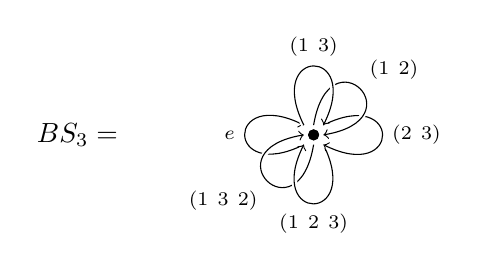
\begin{tikzpicture}
                    \node(BS3)at(0,0){$\cat BS_3=$};
                    % 左侧 S_3
                    \node(dot)at(3,0){\ };
                    \fill (dot) circle [radius=2pt];
                    \draw[color = white, line width = 2pt] (dot.south west) .. controls +(-1,-0.5) and +(-1,0.5) .. (dot.north west);
                    \draw[->] (dot.south west) .. controls +(-1,-0.5) and +(-1,0.5) .. node[left,midway] {{$\scriptstyle e$}} (dot.north west);
                    \draw[color = white, line width = 2pt] (dot.south) .. controls +(-0.2,-1.2) and +(-1.2,-0.2) .. (dot.west);
                    \draw[->] (dot.south) .. controls +(-0.2,-1.2) and +(-1.2,-0.2) .. node[below left,midway] {$\scriptstyle (1\ 3\ 2)$} (dot.west);
                    \draw[color = white, line width = 2pt] (dot.south east) .. controls +(0.5,-1) and +(-0.5,-1) ..  (dot.south west);
                    \draw[->] (dot.south east) .. controls +(0.5,-1) and +(-0.5,-1) .. node[below,midway] {$\scriptstyle (1\ 2\ 3)$} (dot.south west);

                    % 右侧 S_3 的中心对称
                    \node(dot2) at (3,0) {\ };
                    \fill (dot2) circle [radius=2pt];
                    \draw[color = white, line width = 2pt] (dot2.north east) .. controls +(1,0.5) and +(1,-0.5) .. (dot2.south east);
                    \draw[->] (dot2.north east) .. controls +(1,0.5) and +(1,-0.5) .. node[right,midway] {{$\scriptstyle (2\ 3)$}} (dot2.south east);
                    \draw[color = white, line width = 2pt] (dot2.north) .. controls +(0.2,1.2) and +(1.2,0.2) .. (dot2.east);
                    \draw[->] (dot2.north) .. controls +(0.2,1.2) and +(1.2,0.2) .. node[above right,midway] {$\scriptstyle (1\ 2)$} (dot2.east);
                    \draw[color = white, line width = 2pt] (dot2.north west) .. controls +(-0.5,1) and +(0.5,1) ..  (dot2.north east);
                    \draw[->] (dot2.north west) .. controls +(-0.5,1) and +(0.5,1) .. node[above,midway] {$\scriptstyle (1\ 3)$} (dot2.north east);
                \end{tikzpicture}
            \end{center}
            \item 偏序集 \((\cat P,\le)\) (或更一般地说, 预序集) 可视作范畴. \(\cat P\) 的元素即范畴的对象, 而总存在唯一一个态射 \(x\to y\) 当且仅当 \(x\le y\). 偏序关系或者说预序关系 \(\le\) 的传递性蕴含所需态射复合的存在性, 自反性蕴含单位态射的存在性.
            \item 特别地, 任意序数 \(\alpha=\{\beta|\beta<\alpha\}\) 均定义一个范畴, 其对象为那些比之小的序数. 例如, \(\vmathbb0\) 为无任何对象或态射的零范畴, \(\vmathbb1\) 为仅有一个对象且仅有单位态射的平凡范畴,\footnotemark\ \(\vmathbb2\) 则为有两个对象, 同时除单位态射外有一个非单位态射的范畴, 传统上描摹作 \(0\to1\). \(\mathbbpdf{\upomega}\) 为\textit{由图}\[
                \begin{tikzcd}
                    0\ar[r]&1\ar[r]&2\ar[r]&3\ar[r]&\cdots
                \end{tikzcd}    
            \]\textit{自由生成}的范畴, 其中, 任意非单位态射均可唯一分解为上示图中态射的复合. 自由生成的精准定义由例 \ref{441113} 给出.
            \item 集合本身亦可视作范畴, 以集合的元素作为对象, 而态射仅有必需的单位态射. 称某范畴\textbf{离散}当且仅当所有态射均为单位态射.
            \item \(\cat{Htpy}\), 类似 \(\cat{Top}\), 以拓扑空间为对象, 但对象为连续映射的同伦类. 而 \(\cat{Htpy}_*\) 须额外指定基空间、基连续映射的基点保持同伦类.
            \item \(\cat{Measure}\) 以可测空间为对象. 而态射选择为可测函数的等价类, 使得平行的一对函数等价, 当其域的差异为零测集.
    \end{enumerate}
\end{example}\footnotetext{译注: 这里说仅含单位态射, 并非\squarebrace{自然}, 而仅为规定, 反例见前文 \(\cat BG\).}
\par 上述种种, 道尽范畴论之哲学. 例 \ref{Expl:Concrete.Category} 所陈范畴表明数学对象理应连带期间的态射一起探讨, 而列诸 \ref{Expl:Abstract.Category} 者, 又说明态射并非总是函数.\footnote{Reid 的 \textit{Undergraduate algebraic geometry} (《本科代数几何》) 强调, 态射并非总为函数, 原文\cite{Rei88}:\begin{quote}
    \squarebrace{不认可该点的学生建议立即放弃, 转而修读一门范畴论阅读课程.}
\end{quote}} 范畴的态射亦称\textbf{箭头}或\textbf{映射}, 尤其是在例 \ref{Expl:Concrete.Category} 或 \ref{Expl:Abstract.Category} 的背景下.
\begin{remark}
    Russell 悖论蕴含, 没有一个元素为\squarebrace{所有集合}的集合, 此亦定义 \ref{Def:Category} 中采用模糊的\squarebrace{总体}一词之所咎. 事实亦如此, 例 \ref{Expl:Concrete.Category} 中的所有例子, 其对象总体均非集合. Eilenberg 和 Mac~Lane 如下处理这一潜在漏洞:
        \begin{quote}
            ... 整个范畴的概念本质上仅是辅助概念; 我们将基本概念本质上放在\textit{函子}与自然变换上... 范畴的想法仅仅出于每个函数应有固定的类作为定义域和像而必须, 对范畴而言则表现为函子的定义域和像. 所以说范畴这个概念完全可以摒弃, 而尝试构建一个更符直觉的起点, 这里面像\squarebrace{\(\Hom\)}这样的函子就不定义在\squarebrace{所有}群的范畴上,  而仅仅基于可能给定的每个特定的群对. \cite{EM45}
        \end{quote}
    我们面临如此的集合论问题, 定义范畴概念后, 随着范畴理论发展得更远, 这一问题也会随之越发复杂. 基于这等因素, 范畴论学家的常见做法是在 Zermelo-Fraenkel 集合论公理系统的一个扩张里工作, 拥有额外的一些公理去区分\squarebrace{大集合}和\squarebrace{小集合}, 或者集合和类. 为范畴论寻觅最实用的集合论基础, 这一主题亦很迷人, 但很不幸, 这将离开我们的主题太久时间去探索.\footnote{预印本 \cite{Shu08} 给出了激动人心的概述, 不过建议学完本书第 1---4 章后再去阅读.} 相反, 我们把这个问题压到箱底吧, 并不是说这些问题不重要或者无趣, 只是因为其太分散手头任务的注意力了.\footnote{如果不得已必须处理, 假设存在\textbf{不可达基数}的可数序列, 即不可数基数, 它们\textbf{正则}且\textbf{强极限}. 一基数 \(\kappa\) \textbf{正则}, 若所有少于 \(\kappa\) 的基数之并亦小于 \(\kappa\). 而 \(\kappa\) \textbf{强极限}, 若 \(\lambda<\kappa\) 蕴含 \(2^\lambda<\kappa\). 不可达是指小于 \(\kappa\) 的集合在幂集运算与 \(\kappa\)--小并运算下封闭. 若 \(\kappa\) 不可达, 则 von Neumann 层次的 \(\kappa\) 阶段, 即秩小于 \(\kappa\) 的集合之集 \(V_\kappa\), 是带选择公理的 Zermelo-Fraenkel 集合论 (ZFC) 的一个模型; 集合 \(V_\kappa\) 是一个 \textit{Grothendieck 宇宙}. 假设存在一个不可达基数的可数序列, 即可在 \(V_\kappa\) 内部\squarebrace{使用集合论}, 而后根据需要随时扩大宇宙.
    \par 若 ZFC 一致, 那么该公理系统无法证明不可达基数的存在性, 甚至无法证明假设的一致性 (根据 G\"odel 不完备性定理). 尽管如此, 从大基数公理的层垒观点来看, 不可达基数的存在性假设相对比较温和.}
\end{remark}
\par 出于刚刚提及的理由, 有必要介绍用以描述范畴大小的形容词.
\begin{definition}
    称范畴\textbf{小}, 当且仅当其态射总体不超出集合大小.
    \par 由注解 \ref{Rem:CategoryOtherDfntn}, 小范畴的对象总体不超出集合大小. 若 \(\cat{C}\) 是小范畴, 则有映射\[
    \begin{tikzcd}
        \Mor\cat C \ar[r, yshift=.5em, "{\rm dom}"] \ar[r, yshift=-.5em, "{\rm cod}"swap] & \Ob\cat C \ar[l, "{\rm id}"description]
    \end{tikzcd}\]
    递送态射至其域和上域, 而递送对象至其单位态射.
\end{definition}
\par 例 \ref{Expl:Concrete.Category} 中的范畴均非小, 其中每个范畴均携有太多对象. 但\squarebrace{局部而论}, 它们类似于小范畴, 具体陈述如下:
\begin{definition}
    范畴称\textbf{局部小}, 若对所有对象对, 期间的态射总体不超过集合大小.
\end{definition}
    \par 对局部小范畴, 从 \(X\) 到 \(Y\) 的所有态射这一总体习惯上记作\footnote{Mac Lane 赞同 Emmy Noether 所强调的同态在抽象代数中的重要性, 尤其是商群上的同态, 在 Noether 第一同构定理中起了很大作用. 在他回忆中, 箭头记号首次出现于 1940 年, 可能要归因于 Hurewicz \cite{ML88}. 记号 \(\Hom(X,Y)\) 则首次现身于文献 \cite{EM42a}, 用于表示一对 Abel 群间的同态集.}%
    \begin{equation}\label{Eq:Locally.Small.Category}
        \cat C(X,Y)\qquad\text{或}\qquad \Hom(X,Y)
    \end{equation}%
    局部小范畴中, 一对给定对象间的态射集通常称作 \textbf{Hom--集}, 无论其是否任何特定种类的\squarebrace{同态}集. 鉴于 (\ref{Eq:Locally.Small.Category}) 中的记号的确方便
% ! TODO: 环境穿透的脚注自动编号